% !TEX spellcheck = en_US



% ~~~~~~~~~~~~~~~~~~~~~~~~~~~~~~~~~~~~~~~ V
% (NC) 2026 Haluk Bingol
% github.com/halukbingol/LaTeX-Templates
%
% Licensees may copy, distribute, display, and perform the work and make derivative works 
% and remixes based on it only for non-commercial purposes. 
% ~~~~~~~~~~~~~~~~~~~~~~~~~~~~~~~~~~~~~~~ A




% =====================================================================
%  Maven for Java -- Junior Level: Multi-Module Projects, Repositories, Profiles and Rules
%  ---------------------------------------------------------------------
%  Built on hblib/Template/hblibTemplate.tex with the libraries in ../../hblib/.
%  Programs and their real outputs are in codeoutput/:
%     codeoutput/<Name>.java  a program (classes without main() are only compiled)
%     codeoutput/<Name>.sh    a terminal session, run in a copy of codeoutput/<Name>/
%     codeoutput/<Name>.txt   what it printed, made by:  bash run_examples.sh
% =====================================================================

\documentclass[aspectratio=169,10pt,compress]{beamer}

% ~~~~~~~~~~~~~~~~~~~~~~~~~~~~~~~~~~~~~~~~~~~~~~~~~~~~~~~~~~~~~~~~~ V hblib
	\usepackage{../../hblib/hblibPresentation} % lib presentation: theme, i/N, \hSection, algorithm2e, ...
	\usepackage{../../hblib/hblibCodeoutput} % lib code + output: \lstcode, \lstterminal, ...
	\usepackage{../../hblib/hblibDatastructures} % lib data structures: \hString, \hStack, \hQueue
% ~~~~~~~~~~~~~~~~~~~~~~~~~~~~~~~~~~~~~~~~~~~~~~~~~~~~~~~~~~~~~~~~~ A hblib


% theme, i/N, fonts (T1, lmodern), booktabs, xcolor, array (L{width} columns), listings, tikz,
% algorithm2e (\small captions, \Fn) and the color gitred come from the hblib libraries




% +++++++++++++++++++++++++++++++++++++++ V specific
\DontPrintSemicolon % in algorithms
\newcommand{\win}{\textbf{Windows}}
\newcommand{\mac}{\textbf{macOS}}
% +++++++++++++++++++++++++++++++++++++++ A specific

% ---------------------------------------------------------------------
\title{Maven for Java}
\subtitle{Junior Level: Multi-Module Projects, Repositories, Profiles and Rules}
\author[Bingol]{Haluk O. Bingol}

\institute[FCIS]{
    Faculty of Computer and Information Sciences\\
    Yeditepe University
}
\date{
	{\tiny \hbTimeStamp}
}

\begin{document}




% ~~~~~~~~~~~~~~~~~~~~~~~~~~~~~~~~~~~~~~ V frm
\begin{frame}[t,fragile]
  \titlepage
\end{frame}
% ~~~~~~~~~~~~~~~~~~~~~~~~~~~~~~~~~~~~~~ A frm




% ~~~~~~~~~~~~~~~~~~~~~~~~~~~~~~~~~~~~~~ V frm
\begin{frame}[t,fragile] \frametitle{Outline}
  \begin{columns}[T]
    \begin{column}{0.48\textwidth}
      \tableofcontents[sections={1-4}, hideallsubsections]
    \end{column}
    \begin{column}{0.48\textwidth}
      \tableofcontents[sections={5-8}, hideallsubsections]
    \end{column}
  \end{columns}
\end{frame}
% ~~~~~~~~~~~~~~~~~~~~~~~~~~~~~~~~~~~~~~ A frm

% ~~~~~~~~~~~~~~~~~~~~~~~~~~~~~~~~~~~~~~ V
\hSection[Modules]{Multi-Module Projects}
% ~~~~~~~~~~~~~~~~~~~~~~~~~~~~~~~~~~~~~~ A




% ~~~~~~~~~~~~~~~~~~~~~~~~~~~~~~~~~~~~~~ V frm
\begin{frame}[t,fragile] \frametitle{One project, two modules}
  \lstterminal[basicstyle=\ttfamily\tiny]{codeoutput/Layout.txt}

  \vspace{0.1em}
  \small
  \texttt{grades-core}: the logic (\texttt{Course}, \texttt{Gpa}) and its tests; \texttt{grades-app}: a command line program that uses it. One parent \texttt{pom.xml} above both.
\end{frame}
% ~~~~~~~~~~~~~~~~~~~~~~~~~~~~~~~~~~~~~~ A frm




% ~~~~~~~~~~~~~~~~~~~~~~~~~~~~~~~~~~~~~~ V frm
\begin{frame}[t,fragile] \frametitle{The parent: aggregation and inheritance}
  \begin{columns}[T]
    \begin{column}{0.5\textwidth}
      \lstcode[basicstyle=\ttfamily\tiny, firstline=6, firstnumber=6, lastline=30]{codeoutput/Layout/pom.xml}{XML}
    \end{column}
    \begin{column}{0.48\textwidth}
      \begin{itemize}\small
        \item \texttt{<packaging>pom</packaging>}: no code, only configuration.
        \item \textbf{Aggregation}: \texttt{<modules>} builds both with one command.
        \item \textbf{Inheritance}: children get properties, \texttt{dependencyManagement}, \texttt{pluginManagement}.
        \item \texttt{dependencyManagement} fixes versions \emph{without} adding the dependency; a child names only G and A.
      \end{itemize}
    \end{column}
  \end{columns}
\end{frame}
% ~~~~~~~~~~~~~~~~~~~~~~~~~~~~~~~~~~~~~~ A frm




% ~~~~~~~~~~~~~~~~~~~~~~~~~~~~~~~~~~~~~~ V frm
\begin{frame}[t,fragile] \frametitle{A child POM}
  \begin{columns}[T]
    \begin{column}{0.5\textwidth}
      \lstcode[basicstyle=\ttfamily\tiny, firstline=5, firstnumber=5, lastline=18]{codeoutput/Layout/grades-app/pom.xml}{XML}
    \end{column}
    \begin{column}{0.48\textwidth}
      \begin{itemize}\small
        \item \texttt{<parent>}: group and version are inherited; only \texttt{artifactId} is new.
        \item \texttt{grades-core} without a version: it comes from the parent's \texttt{dependencyManagement}.
        \item By default the parent is looked up in \texttt{../pom.xml}, then in the repositories.
        \item Below line 18: the jar manifest (\texttt{mainClass}), as in the sophomore deck.
      \end{itemize}
    \end{column}
  \end{columns}
\end{frame}
% ~~~~~~~~~~~~~~~~~~~~~~~~~~~~~~~~~~~~~~ A frm




% ~~~~~~~~~~~~~~~~~~~~~~~~~~~~~~~~~~~~~~ V frm
\begin{frame}[t,fragile] \frametitle{The reactor (1/2)}
  \lstterminal[basicstyle=\ttfamily\tiny, lastline=20]{codeoutput/Reactor.txt}

  \vspace{0.1em}
  \small The \textbf{reactor} sorts the modules by their dependencies: parent, core, then the app.
\end{frame}
% ~~~~~~~~~~~~~~~~~~~~~~~~~~~~~~~~~~~~~~ A frm




% ~~~~~~~~~~~~~~~~~~~~~~~~~~~~~~~~~~~~~~ V frm
\begin{frame}[t,fragile] \frametitle{The reactor (2/2)}
  \lstterminal[basicstyle=\ttfamily\tiny, firstline=70]{codeoutput/Reactor.txt}

  \vspace{0.1em}
  \small One line per module with its time; the first module that fails stops the rest (\texttt{-fae}: fail at end).
\end{frame}
% ~~~~~~~~~~~~~~~~~~~~~~~~~~~~~~~~~~~~~~ A frm




% ~~~~~~~~~~~~~~~~~~~~~~~~~~~~~~~~~~~~~~ V frm
\begin{frame}[t,fragile] \frametitle{Running the application}
  \lstterminal[basicstyle=\ttfamily\tiny]{codeoutput/RunApp.txt}

  \vspace{0.1em}
  \small
  The app needs both jars on the class path; Windows: \texttt{-cp grades-core\textbackslash target\textbackslash \dots jar;grades-app\textbackslash target\textbackslash \dots jar}. (A shaded jar, sophomore level, avoids this.)
\end{frame}
% ~~~~~~~~~~~~~~~~~~~~~~~~~~~~~~~~~~~~~~ A frm

% ~~~~~~~~~~~~~~~~~~~~~~~~~~~~~~~~~~~~~~ V
\hSection[Repositories]{Repositories}
% ~~~~~~~~~~~~~~~~~~~~~~~~~~~~~~~~~~~~~~ A




% ~~~~~~~~~~~~~~~~~~~~~~~~~~~~~~~~~~~~~~ V frm
\begin{frame}[t,fragile] \frametitle{Building one module}
  \lstterminal[basicstyle=\ttfamily\tiny]{codeoutput/OneModule.txt}

  \vspace{0.1em}
  \small
  Inside \texttt{grades-app} alone, \texttt{grades-core} is not in any repository yet. From the parent: \texttt{-pl} (projects) \texttt{grades-app}, \texttt{-am} (also make) what it needs.
\end{frame}
% ~~~~~~~~~~~~~~~~~~~~~~~~~~~~~~~~~~~~~~ A frm




% ~~~~~~~~~~~~~~~~~~~~~~~~~~~~~~~~~~~~~~ V frm
\begin{frame}[t,fragile] \frametitle{\texttt{mvn install}: into the local repository}
  \lstterminal[basicstyle=\ttfamily\scriptsize]{codeoutput/Install.txt}

  \vspace{0.1em}
  \small
  \texttt{install} copies each jar and POM to \texttt{\textasciitilde/.m2/repository}; now every project on this computer can use \texttt{grades-core}. Windows: \texttt{\%USERPROFILE\%\textbackslash .m2\textbackslash repository}.
\end{frame}
% ~~~~~~~~~~~~~~~~~~~~~~~~~~~~~~~~~~~~~~ A frm




% ~~~~~~~~~~~~~~~~~~~~~~~~~~~~~~~~~~~~~~ V frm
\begin{frame}[t,fragile] \frametitle{Local, remote, mirror}
  \begin{columns}[T]
    \begin{column}{0.46\textwidth}
      \begin{itemize}\small
        \item \textbf{Local} repository: a cache on your disk, \texttt{\textasciitilde/.m2/repository}.
        \item \textbf{Remote}: Maven Central (default), a company repository (Nexus, Artifactory), \dots
        \item Maven asks the local one first, then the remotes; downloads are kept.
        \item \texttt{settings.xml}: per user (\texttt{\textasciitilde/.m2/settings.xml}; Windows \texttt{\%USERPROFILE\%\textbackslash .m2\textbackslash settings.xml}), never in the project: credentials, mirrors, proxies.
        \item This deck ran without internet: \texttt{-s offline-settings.xml} replaces Central by a local copy.
      \end{itemize}
    \end{column}
    \begin{column}{0.52\textwidth}
      \lstcode[basicstyle=\ttfamily\tiny, firstline=7, firstnumber=7, lastline=26]{../offline-settings.xml}{XML}
    \end{column}
  \end{columns}
\end{frame}
% ~~~~~~~~~~~~~~~~~~~~~~~~~~~~~~~~~~~~~~ A frm




% ~~~~~~~~~~~~~~~~~~~~~~~~~~~~~~~~~~~~~~ V frm
\begin{frame}[t,fragile] \frametitle{Source jars for others}
  \lstterminal[basicstyle=\ttfamily\scriptsize]{codeoutput/Sources.txt}

  \vspace{0.1em}
  \small
  \texttt{source:jar} adds \texttt{-sources.jar}: IDEs show the code of a library while debugging. (Libraries for Maven Central also need \texttt{-javadoc.jar}, senior level.)
\end{frame}
% ~~~~~~~~~~~~~~~~~~~~~~~~~~~~~~~~~~~~~~ A frm

% ~~~~~~~~~~~~~~~~~~~~~~~~~~~~~~~~~~~~~~ V
\hSection[Profiles]{Profiles}
% ~~~~~~~~~~~~~~~~~~~~~~~~~~~~~~~~~~~~~~ A




% ~~~~~~~~~~~~~~~~~~~~~~~~~~~~~~~~~~~~~~ V frm
\begin{frame}[t,fragile] \frametitle{Profiles: switchable parts of the POM}
  \begin{columns}[T]
    \begin{column}{0.52\textwidth}
      \lstcode[basicstyle=\ttfamily\tiny, firstline=40, firstnumber=40, lastline=62]{codeoutput/Profiles/pom.xml}{XML}
    \end{column}
    \begin{column}{0.46\textwidth}
      \uncover<2->{\lstterminal[basicstyle=\ttfamily\tiny]{codeoutput/Profiles.txt}}
    \end{column}
  \end{columns}
  \vspace{0.2em}
  \small \texttt{-P prod}: switched on by hand. \texttt{windows}/\texttt{unix}: switched on by the operating system: this run was on Linux (\texttt{unix}); on Windows the file says \texttt{run.cmd}, on macOS \texttt{run.sh}.
\end{frame}
% ~~~~~~~~~~~~~~~~~~~~~~~~~~~~~~~~~~~~~~ A frm




% ~~~~~~~~~~~~~~~~~~~~~~~~~~~~~~~~~~~~~~ V frm
\begin{frame}[t,fragile] \frametitle{Using profiles well}
  \begin{itemize}\small
    \item Good uses: operating system differences, slow integration tests (\texttt{-P it}), a release build (sign, javadoc).
    \item Activation: \texttt{-P id}, \texttt{<activeByDefault>}, a property (\texttt{-Denv=ci}), the JDK version, the OS, a file that exists.
    \item Several at once: \texttt{-P prod,it}; switch one off: \texttt{-P !unix} (in bash: \texttt{-P '!unix'}).
    \item Avoid: a different jar for each environment. Build \emph{once}, configure at run time (environment variables, files).
    \item A build that only works with a secret profile is not reproducible.
  \end{itemize}
\end{frame}
% ~~~~~~~~~~~~~~~~~~~~~~~~~~~~~~~~~~~~~~ A frm

% ~~~~~~~~~~~~~~~~~~~~~~~~~~~~~~~~~~~~~~ V
\hSection[Conflicts]{Version Conflicts}
% ~~~~~~~~~~~~~~~~~~~~~~~~~~~~~~~~~~~~~~ A




% ~~~~~~~~~~~~~~~~~~~~~~~~~~~~~~~~~~~~~~ V frm
\begin{frame}[t,fragile] \frametitle{Two libraries, two versions of a third}
  \begin{columns}[T]
    \begin{column}{0.44\textwidth}
      \begin{center}
      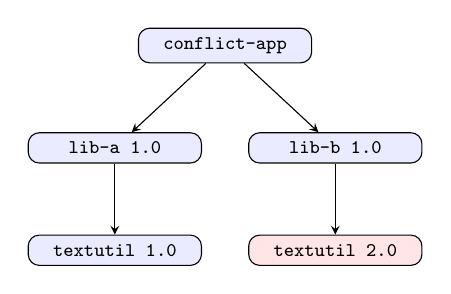
\begin{tikzpicture}[box/.style={draw, rounded corners, fill=blue!8, font=\scriptsize\ttfamily, minimum width=2.2cm}, >=stealth]
        \node[box] (app) at (0,0)      {conflict-app};
        \node[box] (a)   at (-1.4,-1.3) {lib-a 1.0};
        \node[box] (b)   at (1.4,-1.3)  {lib-b 1.0};
        \node[box] (u1)  at (-1.4,-2.6) {textutil 1.0};
        \node[box, fill=red!10] (u2)  at (1.4,-2.6)  {textutil 2.0};
        \draw[->] (app) -- (a);  \draw[->] (app) -- (b);
        \draw[->] (a) -- (u1);   \draw[->] (b) -- (u2);
      \end{tikzpicture}
      \end{center}
      \small \texttt{lib-b} calls \texttt{whisper}, new in \texttt{textutil} 2.0.
    \end{column}
    \begin{column}{0.54\textwidth}
      \lstcode[basicstyle=\ttfamily\tiny]{codeoutput/Conflict/src/main/java/app/Main.java}{Java}
    \end{column}
  \end{columns}
\end{frame}
% ~~~~~~~~~~~~~~~~~~~~~~~~~~~~~~~~~~~~~~ A frm




% ~~~~~~~~~~~~~~~~~~~~~~~~~~~~~~~~~~~~~~ V frm
\begin{frame}[t,fragile] \frametitle{Only one version can win}
  \lstterminal[basicstyle=\ttfamily\tiny]{codeoutput/Conflict.txt}

  \vspace{0.1em}
  \small
  A class path holds one \texttt{textutil}. Both are at depth 2: the \emph{first declared} wins, 1.0. It compiles, and fails at run time: \texttt{NoSuchMethodError}.
\end{frame}
% ~~~~~~~~~~~~~~~~~~~~~~~~~~~~~~~~~~~~~~ A frm




% ~~~~~~~~~~~~~~~~~~~~~~~~~~~~~~~~~~~~~~ V frm
\begin{frame}[t,fragile] \frametitle{The fix: decide the version yourself}
  \begin{columns}[T]
    \begin{column}{0.44\textwidth}
      \lstcode[basicstyle=\ttfamily\tiny, firstline=9, firstnumber=9, lastline=18]{codeoutput/ConflictFix/pom.xml}{XML}
    \end{column}
    \begin{column}{0.54\textwidth}
      \uncover<2->{\lstterminal[basicstyle=\ttfamily\tiny]{codeoutput/ConflictFix.txt}}
    \end{column}
  \end{columns}
  \vspace{0.2em}
  \small \texttt{dependencyManagement} overrides the version everywhere in the tree. Other tools: a direct dependency (nearest wins), \texttt{<exclusions>}.
\end{frame}
% ~~~~~~~~~~~~~~~~~~~~~~~~~~~~~~~~~~~~~~ A frm




% ~~~~~~~~~~~~~~~~~~~~~~~~~~~~~~~~~~~~~~ V frm
\begin{frame}[t,fragile] \frametitle{Let the build find conflicts: enforcer}
  \lstterminal[basicstyle=\ttfamily\tiny]{codeoutput/Convergence.txt}

  \vspace{0.1em}
  \small
  The \texttt{dependencyConvergence} rule fails the build when two paths bring different versions: found at build time, not at run time.
\end{frame}
% ~~~~~~~~~~~~~~~~~~~~~~~~~~~~~~~~~~~~~~ A frm

% ~~~~~~~~~~~~~~~~~~~~~~~~~~~~~~~~~~~~~~ V
\hSection[Rules]{Build Rules}
% ~~~~~~~~~~~~~~~~~~~~~~~~~~~~~~~~~~~~~~ A




% ~~~~~~~~~~~~~~~~~~~~~~~~~~~~~~~~~~~~~~ V frm
\begin{frame}[t,fragile] \frametitle{The enforcer plugin}
  \begin{columns}[T]
    \begin{column}{0.5\textwidth}
      \lstcode[basicstyle=\ttfamily\tiny, firstline=38, firstnumber=38, lastline=54]{codeoutput/Enforcer/pom.xml}{XML}
    \end{column}
    \begin{column}{0.48\textwidth}
      \uncover<2->{\lstterminal[basicstyle=\ttfamily\tiny]{codeoutput/Enforcer.txt}}
    \end{column}
  \end{columns}
  \vspace{0.2em}
  \small Checked at \texttt{validate}, before anything is compiled. Here the rule was raised to Java 25 with \texttt{sed} to show a failure.
\end{frame}
% ~~~~~~~~~~~~~~~~~~~~~~~~~~~~~~~~~~~~~~ A frm




% ~~~~~~~~~~~~~~~~~~~~~~~~~~~~~~~~~~~~~~ V frm
\begin{frame}[t,fragile] \frametitle{Declared what you use?}
  \lstterminal[basicstyle=\ttfamily\scriptsize]{codeoutput/Analyze.txt}

  \vspace{0.1em}
  \small
  \begin{itemize}
    \item \textbf{Used undeclared}: the code calls \texttt{TextUtil} directly but gets it only through \texttt{lib-a}: declare it.
    \item \textbf{Unused declared}: \texttt{commons-lang3} is never used: remove it.
    \item The analysis reads the byte code; reflection and \texttt{runtime} uses may need a manual check.
  \end{itemize}
\end{frame}
% ~~~~~~~~~~~~~~~~~~~~~~~~~~~~~~~~~~~~~~ A frm

% ~~~~~~~~~~~~~~~~~~~~~~~~~~~~~~~~~~~~~~ V
\hSection[Wrapper]{The Maven Wrapper}
% ~~~~~~~~~~~~~~~~~~~~~~~~~~~~~~~~~~~~~~ A




% ~~~~~~~~~~~~~~~~~~~~~~~~~~~~~~~~~~~~~~ V frm
\begin{frame}[t,fragile] \frametitle{Everybody the same Maven: \texttt{mvnw}}
  \begin{itemize}\small
    \item The \textbf{Maven Wrapper}: small scripts in the project that download and use one fixed Maven version.
    \item Created once (needs the internet, not run here): \texttt{mvn wrapper:wrapper -Dmaven=3.10.0}.
    \item It adds \texttt{mvnw}, \texttt{mvnw.cmd} and \texttt{.mvn/wrapper/maven-wrapper.properties}; commit them.
  \end{itemize}
  \begin{columns}[T]
    \begin{column}{0.48\textwidth}
      \begin{block}{Windows (not run here)}


% +++++++++++++++++++++++++++++++++++++++ V lst
%: -Lst.
\begin{lstlisting}[style=codesnippet, language={}, basicstyle=\ttfamily\scriptsize]
mvnw.cmd -v
mvnw.cmd clean verify
\end{lstlisting}
% +++++++++++++++++++++++++++++++++++++++ A lst


      \end{block}
    \end{column}
    \begin{column}{0.48\textwidth}
      \begin{block}{macOS (not run here)}


% +++++++++++++++++++++++++++++++++++++++ V lst
%: -Lst.
\begin{lstlisting}[style=codesnippet, language=bash, basicstyle=\ttfamily\scriptsize]
./mvnw -v
./mvnw clean verify
\end{lstlisting}
% +++++++++++++++++++++++++++++++++++++++ A lst


      \end{block}
    \end{column}
  \end{columns}

  \small \texttt{.mvn/maven.config} can hold options for every build (e.g.\ \texttt{-B -ntp}); \texttt{.mvn/jvm.config} the JVM options.
\end{frame}
% ~~~~~~~~~~~~~~~~~~~~~~~~~~~~~~~~~~~~~~ A frm

% ~~~~~~~~~~~~~~~~~~~~~~~~~~~~~~~~~~~~~~ V
\hSection[Practice]{Good Practice}
% ~~~~~~~~~~~~~~~~~~~~~~~~~~~~~~~~~~~~~~ A




% ~~~~~~~~~~~~~~~~~~~~~~~~~~~~~~~~~~~~~~ V frm
\begin{frame}[t,fragile] \frametitle{A checklist for team projects}
  \begin{columns}[T]
    \begin{column}{0.48\textwidth}
      \begin{itemize}\small
        \item A parent POM with all versions: properties, \texttt{dependencyManagement}, \texttt{pluginManagement}.
        \item Modules by responsibility (core, app, web), dependencies in one direction.
        \item \texttt{mvn clean verify} green before every push.
        \item The wrapper in the repository.
      \end{itemize}
    \end{column}
    \begin{column}{0.48\textwidth}
      \begin{itemize}\small
        \item Enforcer: Java and Maven versions, convergence.
        \item \texttt{dependency:analyze} from time to time.
        \item No secrets in POMs: \texttt{settings.xml} or environment variables.
        \item \texttt{target/}, \texttt{.idea/}, \texttt{.classpath} in \texttt{.gitignore}.
      \end{itemize}
    \end{column}
  \end{columns}
\end{frame}
% ~~~~~~~~~~~~~~~~~~~~~~~~~~~~~~~~~~~~~~ A frm

% ~~~~~~~~~~~~~~~~~~~~~~~~~~~~~~~~~~~~~~ V
\hSection[Summary]{Summary}
% ~~~~~~~~~~~~~~~~~~~~~~~~~~~~~~~~~~~~~~ A




% ~~~~~~~~~~~~~~~~~~~~~~~~~~~~~~~~~~~~~~ V frm
\begin{frame}[t,fragile] \frametitle{Summary}
  \begin{center}\small
  \begin{tabular}{@{}L{0.4\textwidth}L{0.52\textwidth}@{}}
    \toprule
    \textbf{need}                         & \textbf{Maven} \\
    \midrule
    several modules, one build            & parent with \texttt{<modules>}, the reactor \\
    one version for all                   & \texttt{dependencyManagement}, \texttt{pluginManagement} \\
    build part of it                      & \texttt{-pl module -am} \\
    share with other projects             & \texttt{mvn install} (local), \texttt{deploy} (remote) \\
    differences between environments      & profiles (\texttt{-P}, OS, JDK, property) \\
    two versions of one library           & \texttt{dependency:tree -Dverbose}, pin it \\
    rules for the build                   & enforcer \\
    the same Maven everywhere             & \texttt{mvnw} \\
    \bottomrule
  \end{tabular}
  \end{center}
\end{frame}
% ~~~~~~~~~~~~~~~~~~~~~~~~~~~~~~~~~~~~~~ A frm




% ~~~~~~~~~~~~~~~~~~~~~~~~~~~~~~~~~~~~~~ V frm
\begin{frame}[t,fragile] \frametitle{Exercises}
  \begin{enumerate}\small
    \item Add a third module \texttt{grades-report} that prints a transcript table; make \texttt{grades-app} use it. What is the reactor order?
    \item Make \texttt{lib-b} the first dependency in \texttt{conflict-app}; which \texttt{textutil} wins now, and does the program run?
    \item Add a profile \texttt{it} that runs a slow test class only when switched on.
    \item Add the enforcer rule \texttt{requireMavenVersion} \texttt{[3.10,)}; does your own Maven pass?
    \item Run \texttt{dependency:analyze} on a project of yours and fix every warning.
  \end{enumerate}
\end{frame}
% ~~~~~~~~~~~~~~~~~~~~~~~~~~~~~~~~~~~~~~ A frm




% ~~~~~~~~~~~~~~~~~~~~~~~~~~~~~~~~~~~~~~ V frm
\begin{frame}[t,fragile]
	\begin{center}
		\vspace{4cm}
		\hRemark{\Huge Questions?}
	\end{center}
\end{frame}
% ~~~~~~~~~~~~~~~~~~~~~~~~~~~~~~~~~~~~~~ A frm



\end{document}
